\documentclass[a4paper]{article}
\usepackage{float}
\usepackage[english]{babel}
\usepackage[utf8x]{inputenc}
\usepackage{amsmath}
\usepackage{graphicx}
\usepackage{url}
\usepackage{gensymb}
\usepackage[colorinlistoftodos]{todonotes}
\usepackage{fancyvrb}
\usepackage[final]{pdfpages}
%\usepackage[style = ieee, urldate =comp]{biblatex}

\title{Project Hardware Exact Rough Clone Unto Nintendo Entertainment System (Hercu-NES)}
\author{Cody Anderson\\Ben Nollan\\Morgan Skrabut\\Ryan Price}
\date{\parbox{\linewidth}{\centering%
  \today\endgraf\bigskip
  Jeremy Thomas \endgraf\medskip
  Dept.\ of Electrical Computer Engineering \endgraf
  %DigiPen Institute of Technology \endgraf
  \centering{
\includegraphics[width=.65\textwidth]{DigiPenLogo.png}}\endgraf
  ECE 310L, ECE410L, Conjoined \(3^{rd}\) and \(4^{th}\) Year CE Project }}

\begin{document}
\begin{titlepage}
	\maketitle
\end{titlepage}
\begin{abstract}
Project Hardware Exact Rough Clone Unto Nintendo Entertainment System (Hercu-NES) aims to create a Nintendo Entertainment System (NES) clone in SystemVerilog, which will be instantiated on an FPGA. The design of the NES clone will be nearly identical to the design of the actual NES console. In order to create a very similar clone, the discrete IC's on the NES will be modeled by discrete modules in SystemVerilog. Extensive validation and testing will go into checking the correctness of the timing and results of CPU and Picture Processing Unit (PPU) instructions. If we succeed in creating this clone, the Hercu-NES will be capable of running original NES games. 
\end{abstract}

\section{Introduction}
% Clearly state your engineering objective, and how you define success in terms of what your device will do.  Motivate why you want to do this project and provide background information. This should include discussions of your previous work if any, and a brief review of similar work by others in peer reviewed articles.
Remembered and loved by many individuals today, the Nintendo Entertainment System released in North America in 1985 \cite{Nintendo} is a gaming console icon of nostalgia and joyful memories. This console has been brought back to life by few individuals on the FPGA and we propose to achieve the same endeavor this year. We are motivated to recreate the NES ourselves because it is a very rare and highly sought after console with its roots deep in the hearts of many gamers including ours and those of our friends, families, and academic colleagues. We will be referencing two individuals who completed this project themselves (Dan Strother \cite{strother} and Jonathan Ganyer \cite{ganyer}). Our success in completing this project will be defined by our ability to run the game Super Mario Bros. on our FPGA embedded console by the end of the Spring semester.

\section{Methods, Techniques, and Design}
% Describe how you will design and or build your device. Cite references that you consulted on relevant technologies. This should include at least one diagram.
We are going to use an FPGA for this project, an FPGA was chosen over any other platform because it is the most accurate way to replicate the hardware of an NES. It also is much more capable of the task than a similar grade of microcontroller and gives us experience in defining an entire computer system in a hardware description language. We chose to use an Altera DE1 development board because it has enough general I/O accessible for this project. Also, there are already enough of them owned by the college that all the team members can have one. Project Hercu-NES is structured such that the 6502 CPU, the integrated APU, and the PPU each have their own SystemVerilog module and all of these modules will be instantiated on the same FPGA, as a larger NES module. These modules will be connected as though they were all their constituent physical packages. This structure can be seen in Figure \ref{fig:BlockDiagram}. 

\subsection{Block Diagram}
\begin{figure}[H]
\centering
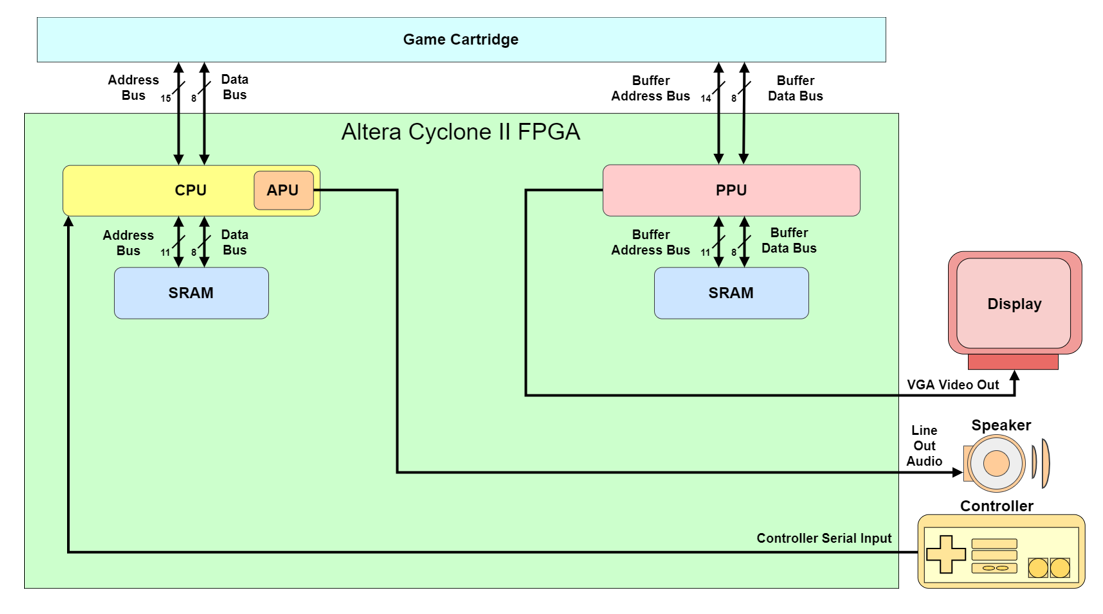
\includegraphics[width=\textwidth]{Capture.PNG}
\caption{\label{fig:BlockDiagram}Project Block Diagram showing simplified flow of data and physical structure of components and modules}
\end{figure}

\subsection{Central Processing Unit (CPU)}
The CPU in the NES is based on the 6502 CPU, but with a few changes. The CPU operates at a frequency of 1.79 MHz and the Audio Processing Unit (APU) is built into the same package. In terms of I/O, the CPU has a 16-bit address bus and a bi-directional 8-bit data bus.\cite{nesdev}

\subsection{Picture Processing Unit (PPU)}
The NES PPU is used for generating two-dimensional scenes by using composite video output. It operates at 21.48 Mhz and outputs one pixel per clock cycle. It also has a dedicated 2K SRAM Chip for storing data which is shown above in Figure 1 below the PPU. This chip communicates with the CPU by using the CPU data bus. It also is connected to three of the CPU address lines, these are used to select the PPU register.\cite{nesdev} Sprites on the NES are limited to either 8x8 and 8x16 pixels which makes things fairly simple for our purposes. The PPU implements a type of scrolling in order to show larger worlds than the display's resolution alone can show. It does so using PPU internal registers which are 1-15 bits long that allows the PU to read and write to memory in order to draw the background and update the data of what is being drawn.\cite{nesdev} This process will be more complicated in a splitscreen setting but that is not yet in our list of goals. 

\subsection{Chip Interconnects}
In the NES, all of the devices share the data lines and take turns outputting to them. This method won't work when using SystemVerilog to describe the hardware as it doesn't have the capability to resolve multiple driving nets. The current solution that we intend to use is the method of separating the inputting and outputting of each device. Then all the data buses will be passed through a multiplexer. This system should mitigate some of the issues with multi driver nets and shouldn't pose any problems with data propagation.

\subsection{Hardware Interface}
We are going to connect a cartridge interface and two controllers to the FPGA using the two 40-pin expansion ports on the FPGA. The cartridge is a 72-pin socket, most of which are used. Each controller connector has 7 pins, four of which connect to the CPU data bus.\cite{nesdev}

A NES cartridge has 72 pins, but not all will be needed for this implementation. The CIC (Checking Integrated Circuit) system occupies four pins on the cartridge: two data buses, a clock line, and a reset line. Since the CIC system will not be implemented in this design, all four of those pins can be excluded. Ten expansion port pins are also present on a NES cartridge. These expansion port pins would have been used to connect to third party accessories, however no commercial products were ever developed that utilized the port (with the exception of the many accessories made for the Japanese version of the NES, the Famicom)\cite{EXport}. These expansion port pins will also be excluded from this implementation, reducing the total amount of pins utilized by the cartridge to 58.

A standard NES controller has five pins: +5v, data clock, data latch, serial data, and ground \cite{controller}. The ground and power pins can be shared between the two controller inputs, bringing the total number of pins for two controllers down to seven pins. This means that a NES cartridge and two controllers can interface to the FPGA using a total of 65 pins, which is less than the 80 pins we have available through the 80 pins on the Altera DE2's expansion ports.

\subsection{Audio Processing Unit (APU)}
The APU is made up of five output channels. These channels include:
	\begin{itemize}
    	\item Two (2) square wave generators
        \item One (1) triangle wave generator
        \item One (1) sample generator
        \item One (1) noise generator
    \end{itemize}
    Each of these channels are fed into their own DAC. Each channel is then combined in the APU Mixer. The APU Mixer is an analog circuit, but can be approximated easily with digital logic.\cite{nesdev}


\section{Schedule and Task Breakdown}
% Presents a detailed breakdown of the schedule into weekly tasks and first and second milestones with measurable goals.

As you can see in Figure 2, we each have one distinct job in this project. The task distribution among team members will go as follows:
\begin{itemize}
\item Cody Anderson is in charge of overlooking the task of CPU creation \\
\item Morgan Skrabut is in charge of overlooking the task of PPU creation \\
\item Ryan Price is in charge of the cartridge and controller connectivity as well as the APU \\
\item Ben Nollan is in charge of designing module framework and all testing and verification
\end{itemize}
First Half Semester Milestones (Week 7):
\begin{itemize}
\item Have Framework Completed. \\
\item Implement internal registers of CPU. \\
\item Basic video output of PPU. \\
\item Cartridge to FPGA connectivity. \\
\end{itemize}
Second Half Semester Milestones (Week 12):
\begin{itemize}
\item Basic CPU functionality working (some opcodes execute correctly). \\
\item Some audio outputting. \\
\item Background Color and one or more sprite rendering. \\
\item Complete controller and cartridge connectivity. \\
\end{itemize}
\begin{figure}[H]
\centering
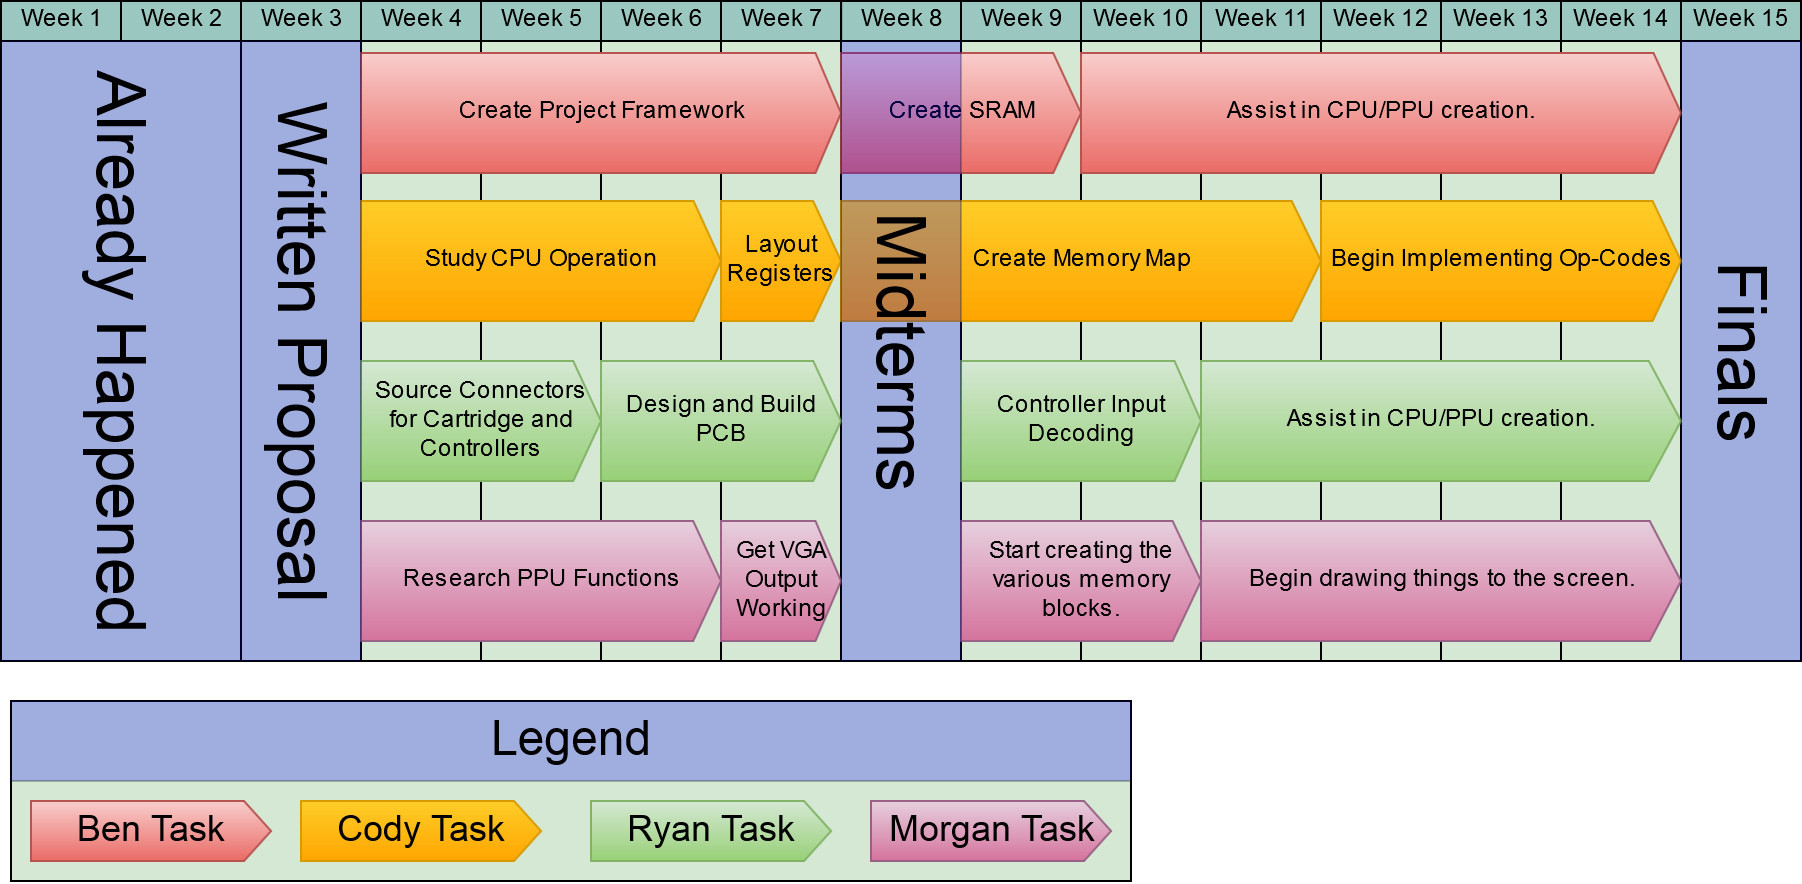
\includegraphics[width=\textwidth]{Schedule.png}
\caption{\label{fig:Schedule}Project task breakdown for this semester.}
\end{figure}

\section{Bill of Materials}
As you can see below in Figure 3, our bill of materials includes the DE2 boards, a system and some of its official accessories, some connectors and other necessary pieces. First off, we already have some DE2's readily available to us so those don't need to be purchased. Then we decided we need an NES and games because we will be using the official system and its accessories to test, verify, and design our own version of the NES. Lastly, we'll need cables and connectors in order to be able to use the official cartridges on our own FPGA system which is part of our end-goal. 
\begin{figure}[H]
\centering
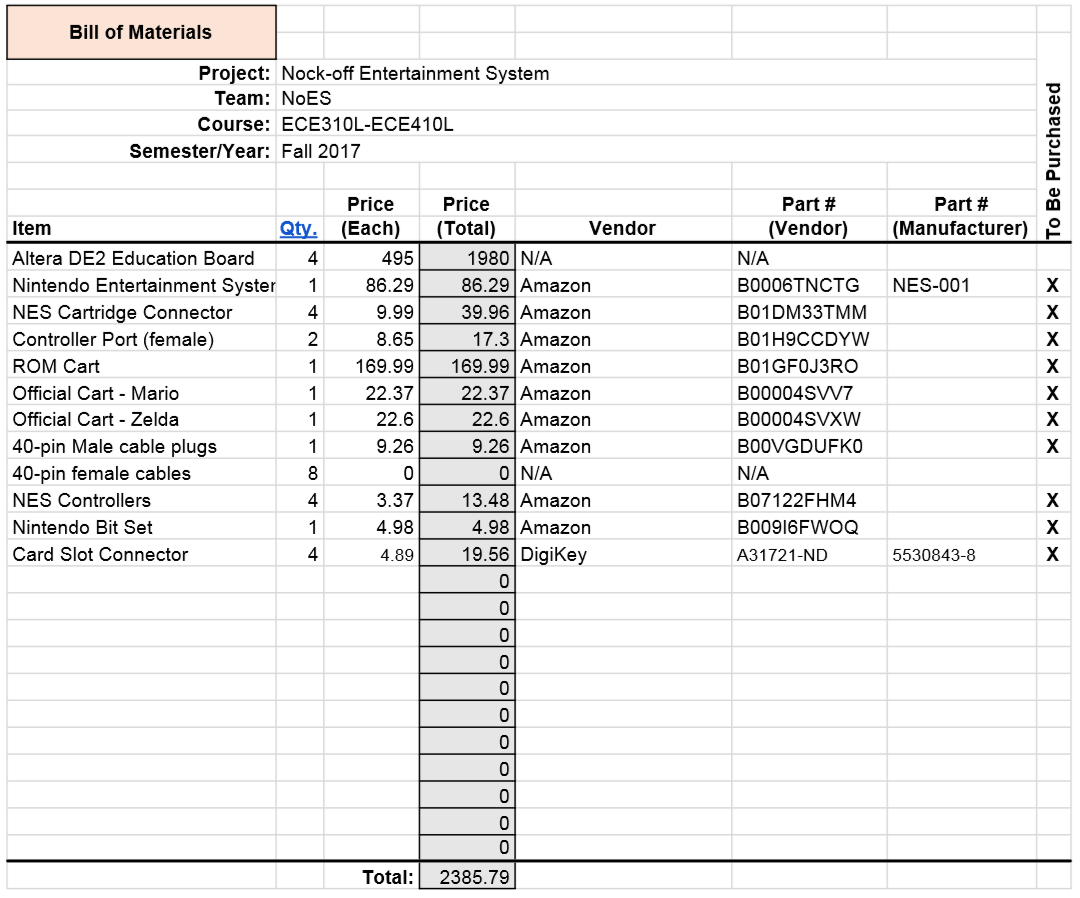
\includegraphics[width=\textwidth]{bom.png}
\caption{\label{fig:Table}Project Bill of Materials}
\end{figure}

%\section{Testing and Design Verification}
%Present data and/or observations showing how you verified the functionality of your device. Include graphs, tables, diagrams, etc. The data should be presented objectively. Save any discussion for the Discussion section.

%\section{Discussion}
%Discuss implications of the design verification data for your engineering objective. The discussion should address questions or goals presented in your introduction. 

%\section{Conclusions and Future Work}
%Summarize your results and briefly describe future studies that could continue or improve this work.  

% \section{Acknowledgements}
% %Briefly thank people who helped you work on this. DO NOT INCLUDE REFERENCES HERE. 
% 	A special thanks to:
%     \begin{itemize}
%     	\item Jeremy Thomas
%         \item Lukas VanGinneken
%         \item Nick Rivera
%         \item 
        
%     \end{itemize}

% \section{Author Contributions}
% %Include a statement of responsibility that specifies the contribution of every team member. Examples of published "author contributions" statements can be seen at http://blogs.nature.com/nautilus/2007/11/post_12.html 
% 	\begin{itemize}
%     	\item Ben's Acts:
%         \begin{itemize}
%         	\item HDMI Input
%             \item Monitor Identification
%         	\item TMDS Decoding
%         	\item TMDS Encoding
%         	\item HDMI Output
%             \item RGB to HSV
%             \item HSV to RGB
%         	\item Division Pipelining
%         \end{itemize}
        
%     	\item Cody's Acts:
%         \begin{itemize}
%         	\item HSV Transformation Prototyping
%         	\item XYZ Transformation Prototyping
%             \item Colorblindness Simulation Prototyping
%             \item Colorblindness Correction Prototyping
%             \item RGB to HSV
%             \item HSV to RGB
            
%         \item All authors contributed equally to this paper.
%         \end{itemize}
% 	\end{itemize}


% You must cite all references that you significantly consulted for the writing of the proposal in IEEE format in the bibliography. In addition, for all quoted material the source must be referenced. This includes figures, charts and tables that were obtained from other papers.

%\cite{ganyer}
%\cite{nesdev}
%\cite{strothe}

\bibliographystyle{IEEEtran}
\bibliography{bibliography.bib}

\end{document}